\documentclass{article}
\usepackage{amsmath} % Ajouter dans le préambule si nécessaire
\usepackage{graphicx} % Required for inserting images
\usepackage{hyperref} % Required for inserting hyperlinks
\usepackage{float}

\title{Automatic detection of hyperparameters in datasets \\
       \large Predictions for nearest neighbor models}
%\subtitle{Prediction of the KNN hyperparameter}
\author{Alexis Rosenfeld \& François Delafontaine}
\date{Fall 2024}

\begin{document}

\maketitle

\section{Research Question and Motivation}
% usual hyperparameter retrieval method through accuracy iteration
% deriving the parameter from dataset characteristics (dependent variables)
% limitation to kNN models
In this project, we will work on the KNN algorithm and more specifically on its only hyperparameter, 'k'. But what are hyperparameters? The scikit-learn documentation defines hyperparameters as: “aspects for configuring model structure that are often not directly learned from data.” Because ML algorithms tend to consider many data dimensions, we understand that mathematically modeling the optimal parameters of models, the hyperparameters, is not an easy task. The phrase “often not directly learned” highlights the common way to find them: experimentation.

Nevertheless, we observe that for simple ML models like KNN, links between “the data” and the hyperparameter 'k' exist. More formally, we can easily imagine a relationship between the distribution of the data's dimensions and 'k'. For example, the proximity between the distributions of different categories' features:

\begin{figure}[H]
	\centering
	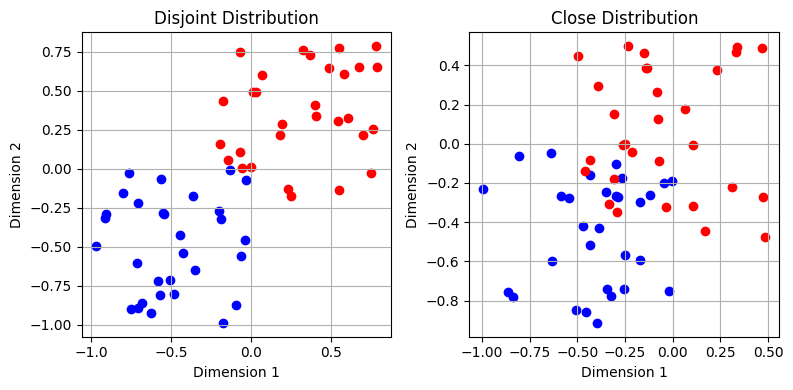
\includegraphics[scale=0.45]{Img/il1.png}
	\label{fig:csehr}
    \caption{Link between optimal k and the distribution of features across categories (k=1 in the first case but k=3 in the second case due to the "closeness" of the parameter's distributions among the categories)}
\end{figure}

Our question now is: how can we, using ML, formalize the relationship between dataset statistics and 'k'?

\section{Dataset}

We create a dataset \( D = y + X \), where \( y \) is the label of our model and \( X \) is the matrix of predictors. We then use cross-validation to estimate the best \( k \) value.
\\[0.2cm]
We are then able to build our target dataset \( D_t = y_k + X_s \), where \( y_k \) represents the different values of \( k \) we found for our dataset \( D \) using different \( X \), whose statistics become the new matrix parameters \( X_s \).
\\[0.2cm]
\( X_s \) could, for instance, be formed from the proximity between the distributions of different categories' features, the noise of the features, or the number of data points in the features.
\\[0.2cm]
Formally, we could hypothesize:
\begin{itemize}
\item The closer the distributions of different categories' features, the higher the \( k \) value.
\item The more \textit{noise} a dataset has, the higher the 'k' value.
\item The more data points a dataset has, the higher the 'k' value.
\item Regarding data length, we can confirm a \textit{rule of thumb} (\href{https://stackoverflow.com/questions/11568897/value-of-k-in-k-nearest-neighbor-algorithm}{StackOverflow}, 16.10.2024): \( k = \sqrt{n}/2 \).
\end{itemize}

To summarize, the dataset \( D_t \) is generated thanks to the optimal KNN hyperparameter of various \( D \) generated using arbitrary \( y \) and \( X \) defined according to some distributional features and statistics found in \( X_s \).

\section{Model}

Due to the nature of our 'y', with the number of values unknown, we should only consider a regression model (with the output rounded). We have already defined the basic model:

$$ k  =  \text{distribution closeness} + \text{noise} + \text{data length} $$

Once relevant variables have been identified, along with a formula to relate them to 'k', the focus should be on refining that model.

\section{Discussion (Problems)}

Our observation so far is that the 'k' value should vary widely, and, therefore, our dataset should be challenging, resulting in our model's precision being relatively poor. To evaluate the model, we should not only check if the value is exact but also how close our predicted value is to the actual optimal 'k' value.

\end{document}